\chapter{Related Work} \label{cpt-related-work}

The proposed approach is an aggregation of a lot of ideas and implementations that have been 
around for quite some time. It is of great interest to explore related work, which can provide 
context for use cases and highlight additional techniques that can be adopted additionally. 
This chapter highlights related work addressing \emph{Voxel Rendering}, \emph{Occlusion Culling}, 
and \emph{Mesh Shading}, on which the proposed implementation is based. The most important of 
the highlighted concepts are revisited and discussed in more detail in chapter 
\ref{cpt-technical-background}. 

[@TODO: Find scientific papers for voxel representations]

\section{Voxel Representation} \label{sec-voxel-representation}

\begin{figure}[h]
    \centering
    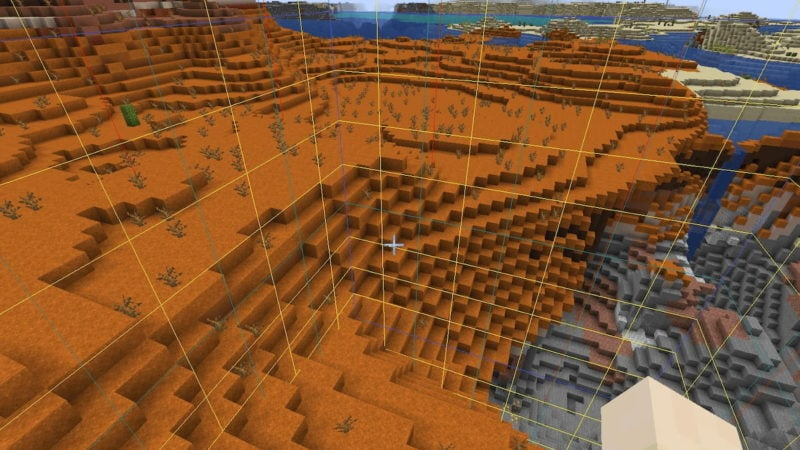
\includegraphics[width=300px]{images/graphics/minecraft-chunks.jpg}
    \caption{A screenshot from \emph{Minecraft}, with a debug visualization of the voxel chunks \cite{Palm2022}.}
    \label{fig:minecraft-chunks}
\end{figure}

\noindent
Voxel Rendering has had huge success in sandbox and highly dynamic games like \emph{Minecraft} (Mojang 
\cite{Mojang2024}, 2011) or \emph{Teardown} (Tuxedo Labs \cite{TuxedoLabs2022}, 2022). Usually these games try 
to preserve some volumetric information for the dynamic environment to be manipulated in real-time. \emph{Minecraft} 
generates a procedural environment based on complex parameters. This way, they can easily generate nearly infinite 
worlds with interesting biomes and landmarks. This huge world is split into chunks of size 16×384×16, to be able to 
stream the world dynamically and allow for quick traversal in any direction, shown in figure \ref{fig:minecraft-chunks}.
Each chunk maintains its own three-dimensional grid, with the voxel data being highly compressed. Non-existing voxels 
are not being stored, and block states, textures, and other information is stored in per-chunk buffers or as global 
data in a global buffer. This way, using a texture atlas, up to 256 different texture variants can be easily stored 
per voxel by only one byte \cite{Bergensten2012, MinecraftFandom2021}. \\

\noindent
Many other games have made use of voxel rendering, adapting these principles of data compression and data streaming. 
Most optimizations rely on culling voxels, which are not visible, e. g. faces that touch other faces.
Frustum culling and occlusion queries are also part of the optimization process and partially used in \emph{Minecraft} 
as well, though the existence of frustum culling or the specific occlusion culling algorithm added in version 1.5 
cannot be confirmed finally and reliably. Nevertheless, many efforts towards better performance have been made on the 
\ac{CPU} side. Lately, \ac{GPU}-driven approaches have been implemented by various individual developers. 
[@TODO: Find specific optimizations and sources!]  \\

\begin{figure}[h]
    \centering
    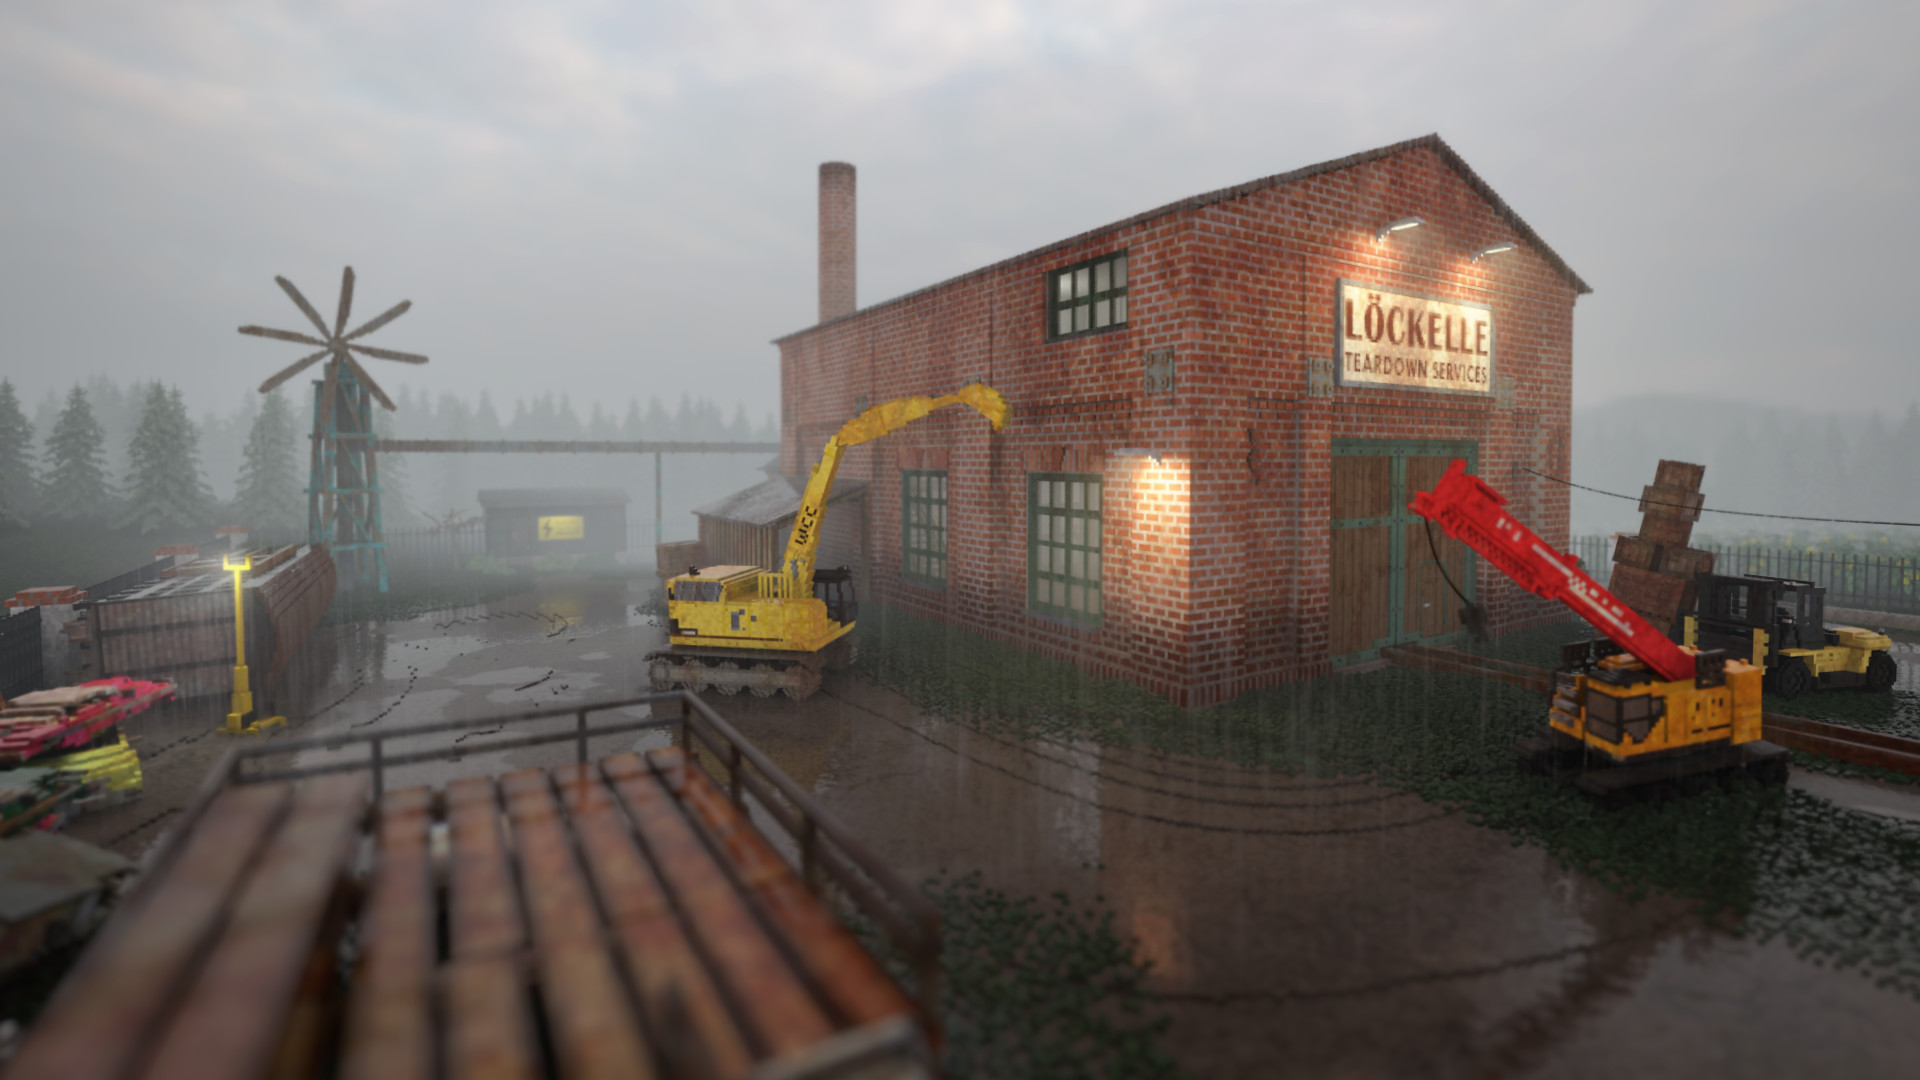
\includegraphics[width=300px]{images/graphics/teardown-ray-tracing.jpg}
    \caption{A screenshot from \emph{Teardown}, showcasing raytraced lighting \cite{TeardownSteam2022}.}
    \label{fig:teardown-raytracing}
\end{figure}

\subsection*{Efficient Sparse Voxel Octrees}

Laine and Karras \cite{Laine2010} analyze and implement a variation of the base Sparse Voxel Octree approach for 
raytracing voxel models. In their work, contours are used to approximate octree nodes within a \ac{SVO}. If the 
octree node is found to be apprixamted good enough, the subdivision to deeper levels in the octree node is terminated
\cite{Kampe2013,Laine2010}. This way, \ac{SVO}s can be significantly reduced in size, which benefits the memory 
footprint of the application. \\

\noindent
The efficient \ac{SVO}s feature a similar approach to this work in that octree nodes are approximated for faster 
processing times. While Laine et al. use contours for their approximations, this work uses whole octree nodes 
to approximate volumes. \\

\noindent
However, Laine et al. use their implementation for raytraced voxel rendering and the approximations are targeting 
model boundaries only instead of volumes. Therefore, the approximation using contours is not aiming for the same 
optimization than this work's approximation does. While the first one refers to optimizing ray casting, the latter 
refers to optimizing a depth prepass computation.. Nevertheless, both approaches share the aspect of reducing 
octree complexity by approximating parts of the tree hierarchy.


\subsection*{Sparse Voxel Directed Acyclic Graphs}

Kämpe et al. \cite{Kampe2013} propose the use of their \emph{High-Resolution Sparse Voxel \ac{DAG}s}. This approach 
is tailored to high voxel resolutions and data that might not fit into memory all at once. Their data structure can 
be easily split up into several sub-trees, which in turn can be loaded individually. This approach seems promising 
for large scenes and use cases, which require the streaming of data. They propose to structure the data in a way that 
enables equal nodes of an octree hierarchy to be reduced to only one instance, eliminating redundant parts of the 
hierarchy and reducing the amount of used memory immensely. \\

\noindent
This approach relates to this implementation in how large voxelized scenes can be efficiently loaded and stored in 
memory. Although this work doesn't explicitly rely on Sparse Voxel \ac{DAG}s, Sparse Voxel octrees are used in the 
provided implementation. Additionally, the proposed implementation can be optimized in the future to be working 
with Sparse Voxel \ac{DAG}s, enabling the handling of meshes with even higher resolution. \\

\noindent
Sparse Voxel \ac{DAG}s are not commonly used in rasterized rendering pipelines and store voxlumetric data in a binary 
format instead of storing positional data. This introduces additional complexity to the pipeline, which might result in 
better runtime performance but is also less intuitive when dealing with nodes and individual voxels. Sparse Voxel 
\ac{DAG}s mainly aim to provide a smaller memory footprint for raytraced applications while maintaining high resolution 
voxel meshes. \\

\noindent
Compared to this work's approach, Sparse Voxels \ac{DAG}s are able to resolve voxel data more efficiently and is 
better suited for higher resolution meshes that might exceed memory limits in a raw data format. However, their 
primary usage is ray-traced rendering which is not what this work is concerned with. While Sparse Voxel \ac{DAG}s 
could generally be applied to rasterized rendering, this work uses a custom Sparse Voxel Octree, optimized for 
traversal and easy coordinate extraction. 


\section{Occlusion Culling}


\subsection*{Hierarchical Z-Buffering}

Greene et al. \cite{Greene93,Greene95} proposed the first \ac{HZB} algorithm with the capability to use screen space 
data to cull meshes in large and densely populated scenes. The idea originated in the context of a forward rendered 
pipeline, making use of the \ac{CPU} for culling instances. They propose to use a spatial container like an octree to 
enable drawing the scene in a rough front-to-back order. Each mesh is individually drawn to a depth buffer resource, 
starting with an empty one in the beginning and populating it as more meshes are drawn. The buffer resource also 
maintains a mip chain that is updated when the full resolution depth buffer is updated. Each time a mesh is rendered 
to the depth buffer, it is checked against the depth hierarchy, starting with the coarsest mip level. This way, near 
and big objects are likely to occlude small, far objects, resulting in an efficient way to reject invisible meshes.\\

\noindent
Although this technique was intended for use on the \ac{CPU}, it can be easily adapted to work on \ac{GPU} resources 
without the need of a write-back to expose the data to \ac{CPU} memory. The approach by Greene et al. is the basis for 
modern \ac{GPU} based algorithms and a major influence for the work at hand. It uses the same principle of hierarchical 
visibility testing and maintaining a depth buffer. \\

\noindent
However, more modern approaches are used to adapt this algorithm for \ac{GPU} friendly design, like computing the depth 
in a pre-pass, using only best occluders instead of all possible meshes, and disabling color writes completely. This also 
limits the amount of recomputations of the mip-chain since all occluders are only drawn to the depth buffer once per 
frame instead of scaling with the number of visible meshes.

\subsection*{Umbra}

In the past, occlusion culling in games has been heavily influenced by \emph{Umbra} \cite{Umbra2024}, a company 
specializing in 3D occlusion culling solutions. \emph{Umbra} has been used by a lot of games such as 
\emph{Call of Duty: Ghosts} (2013), \emph{Killzone: Shadow Fall} (2013), \emph{Alan Wake} (2012), and many more 
\cite{UmbraWiki,CallOfDutyGhostsCredits,KillzoneUmbra,AlanWakeUmbra}. \\

\noindent
\emph{Umbra} voxelizes the game world and proceeds to process the data further, merging voxels into cells. 
A runtime hierarchy of the meshes inside the voxelgrid is created and subsequently, using the camera position, 
the cells can be queried for occlusion. As long as there are large occluders, this process can reduce the number 
of instances and therefore the number of triangles to draw. \emph{Umbra} also keeps a simplified depth buffer in 
memory in order to quickly determine visibility \cite{Medium2018}. \\

\noindent 
The approach is similar to the approach provided  in this work, in that both use a depth buffer and a scene hierarchy 
for computing visibility early in the pipeline. Both approaches rely on screen-space bounding comparisons, although 
\emph{Umbra} uses a \emph{Portals and Cell} structure to manage visibility testing for a given camera position 
\cite{Medium2018}. Furthermore, \emph{Umbra} is usually applied in triangle mesh scene representations instead 
of volumetric, voxel-based scene representations. \emph{Umbra} uses runtime data structures for efficient visibility 
optimizations based on static scene meshes, while this work uses octree queries to dynamically determine possible 
occluders during runtime - or as a one-time pre-computation for voxel models that are known to be static. \\


\subsection*{Two-Pass Occlusion Culling}

\noindent [@TODO: Remove AC Unity and only focus on Aaltonen]
\emph{Assassin's Creed Unity} (2014) uses a \ac{GPU} based two-pass occlusion culling technique as presented by 
Aaltonen et al. \cite{Aaltonen2015}. This technique involves both \ac{HZB} and depth reprojection. Both make for 
a good occlusion culling technique in games with large occluders or interiors. First, artist picked 
\emph{best occluders} are drawn to the depth buffer in a depth pre-pass. Then, projected bounding boxes can be 
used to test the visibility of smaller objects in the scene. A hierarchical z-buffer is used to accelerate this 
testing, as proposed by Greene et al. \cite{Greene93,Greene95}. Finally, the depth buffer of the last frame can be 
reprojected to further minimize computations. This technique allows developers to push for huge draw distances and 
densely crowded environments.\\

\noindent
Similar to this work, the game uses advanced technology in its implementation, clustering geometry, and allowing 
for a \ac{GPU} centric approach to occlusion culling. However, the game doesn't use a volumetric representation 
but the standard boundary representation for its world. Furthermore, the best occluders are provided in different 
ways. Aaltonen et al. \cite{Aaltonen2015} propose the use of a hand-picked set of large, static meshes, while this 
work relies on a simple approximation of the voxel layout. This way, the latter implementation can dynamically 
provide best occluders during runtime, adapting the occlusion capabilities with the addition or removal of voxels 
in the scene.


\subsection*{Masked Software Occlusion Culling}

Hasselgren et al. \cite{Hasselgren2016} present a novel way of implementing occlusion culling relying on hardware 
occlusion queries while optimizing the queries using \ac{CPU} \ac{SIMD} acceleration. The basic algorithm is very 
similar to common \ac{CPU} or \ac{GPU} computed \ac{HZB}, with two major alterations to the implementation. First, 
they make use of Intel's \ac{AVX} to compute depth values for tiles of 256 texels in parallel. The second difference 
is the way they store depth and coverage data. In contrast to a "normal" \ac{HiZ} mip-chain, Hasselgren et al. 
decouple depth and coverage data by storing a coverage mask for \begin{math}32 \times 8\end{math} pixel tiles, 
which can be efficiently computed by using the \ac{AVX} of Intel \ac{CPU}s. In their results, they show that their 
implementation is up to 3 times faster than previous occlusion culling algorithms while also providing a lower 
memory footprint. \\

\noindent
The work of Hasselgren et al. relates to this work's implementation in the general concept of occlusion culling, making 
use of projected bounding boxes, and a comparison of minimal z values. Their work shows that such an algorithm can be 
optimized for \ac{CPU} execution using \ac{SIMD} and effective use of data structures. \\

\noindent 
In contrast to this work, Hasselgren et al. use their algorithm for non-volumetric triangle meshes. This means that 
they make heavy use of raster occlusion queries, making rendering CPU-bound. While still efficient and possibly faster 
than \ac{HZB}, Masked Software Occlusion Culling lacks the \ac{GPU} driven basis for this work's implementation. This 
work's approach does not work with geometry on the \ac{CPU} side at all but leaves all of the triangle computations up 
to the last possible stage of the pipeline, making the application of \ac{CPU} accelerated occlusion queries impractical.


\subsection*{Per-Meshlet Two-Pass Occlusion Culling}

Similar to \emph{Assassin's Creed Unity}, the game \emph{Alan Wake 2} (2023) and engine \emph{Unreal Engine 5} also 
implement \ac{HZB} and depth reprojection. Both implementations are directly based on the approach of Aaltonen et 
al. \cite{Aaltonen2015}, but this time, making use of the new \emph{Mesh Shading} pipeline. The difference being the 
now provided hardware integration of clustering geometry \cite{Remedy2023,Karis2021}.  \\

\noindent
Karis et al. and Remedy Entertainment find that using \ac{HZB} can provide great runtime performance for open, 
highly dense scenes. Both combine the \ac{HZB} with depth reprojection to further optimize the computation of the 
depth buffer. Using the Mesh Shading pipeline, this concept can be applied to meshlets, enabling per-meshlet culling. 
That means that small parts of the geometry can be culled, even if other parts of the same mesh are still visible. 
This optimizes the culling further so scenes can be more densely populated with meshes.\\

\noindent
The findings of Karis et al. and Remedy Entertainment are adapted for this work's implementation, which also relies on 
the use of the Mesh Shading pipeline. While the implementations of Karis et al. and Remedy Entertainment are based on 
a boundary representation and do not require the use of a spatial container for the culling algorithm, this 
implementation aims for a different use case. Contrary to boundary representations, the spatial properties of voxels 
can be used to approximate volumetric coverage by less complex geometry, making it more efficient to select and draw 
best occluders. Also, this work uses the best occluders not only to occlude meshlets, which are behind the best occluders, 
but it can additionally be used to occlude parts of the best occluders itself. This poses a new way of applying occluders 
in the context of rendering volumetric scenes.


% SV DAGs
% AC Unity
% Alan Wake 2
% Greene
% Raster OC using depth queries -> not viable for so many objects